\section{Measurement}
\begin{frame}{Ge--76-Detectors}
	\begin{itemize}
		\item Germanium can serve as a semiconductor detector $\Rightarrow$ source and detector at the same time
		\item Natural abundance of Ge-76: \SI{7.44}{\percent}, detector is a high purity single crystal
		\item Has to be cooled to \SI{90}{\kelvin} and shielded against background radiation
		\item $Q=m\l({}^{76}_{32}Ge\r)-m\l({}^{76}_{34}Se\r)=\SI{2039.006}{\kilo\electronvolt}$\footnotemark[1]
		\item $0\nu\beta\beta$ decay has experimentally nice signature: peak at $Q$
		\item $0\nu\beta\beta$ single site event (SSE) are selectable by pulse-shape
	\end{itemize}
	\vspace{-3em}
	\begin{figure}[]
		\hbox{\hspace{25em}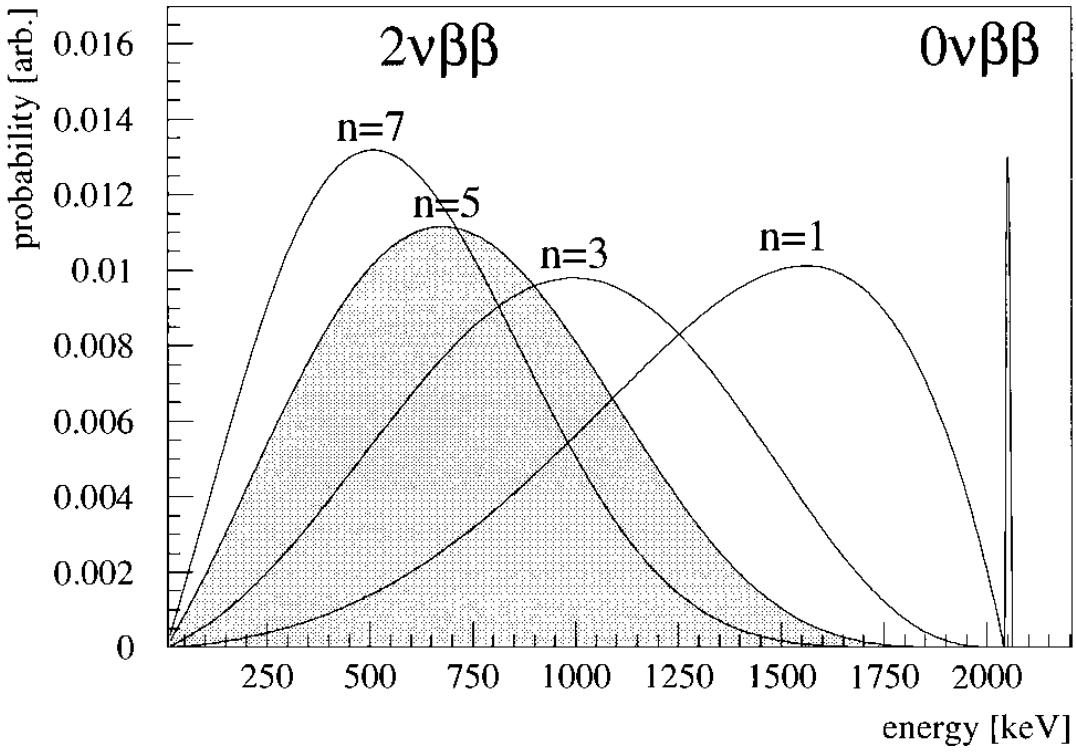
\includegraphics[width=0.37\linewidth]{media/spectrum.png}}
		\caption*{\hspace{25em}Signal Shape\footnote[2]{\fullcite{HMFull}}}%
	\end{figure}
	\vspace{-4em}
	\footnotetext[1]{\fullcite{Qval}}
\end{frame}
\begin{frame}
	\frametitle{The Heidelberg-Moscow Experiment}
	\begin{itemize}
		\item located at the underground labratory at \emph{Gran Sasso (LNGS)} (equiv. \SI{3.500}{\meter} water)
		\item \SI{11.5}{\kilo\gram} Ge-76 enriched to \SI{86}{\percent} Ge-76 (Devided into 5 detectors) $=\SI{125.5}{\mole}$
		\item Assembeled in close to clean-room conditions
		\item Shielding: \SI{10}{\centi\meter} radiopure $\symup{Pb}+\SI{20}{\centi\meter}\ \symup{Pb}+$ pressurized liquid $\symup{N}+\SI{10}{\centi\meter}$
		      boron loaded polyethylene
		\item $\symup{FWHM}\approx\SI{3}{\kilo\electronvolt}$
	\end{itemize}

	%\begin{figure}
	%	\centering
	%	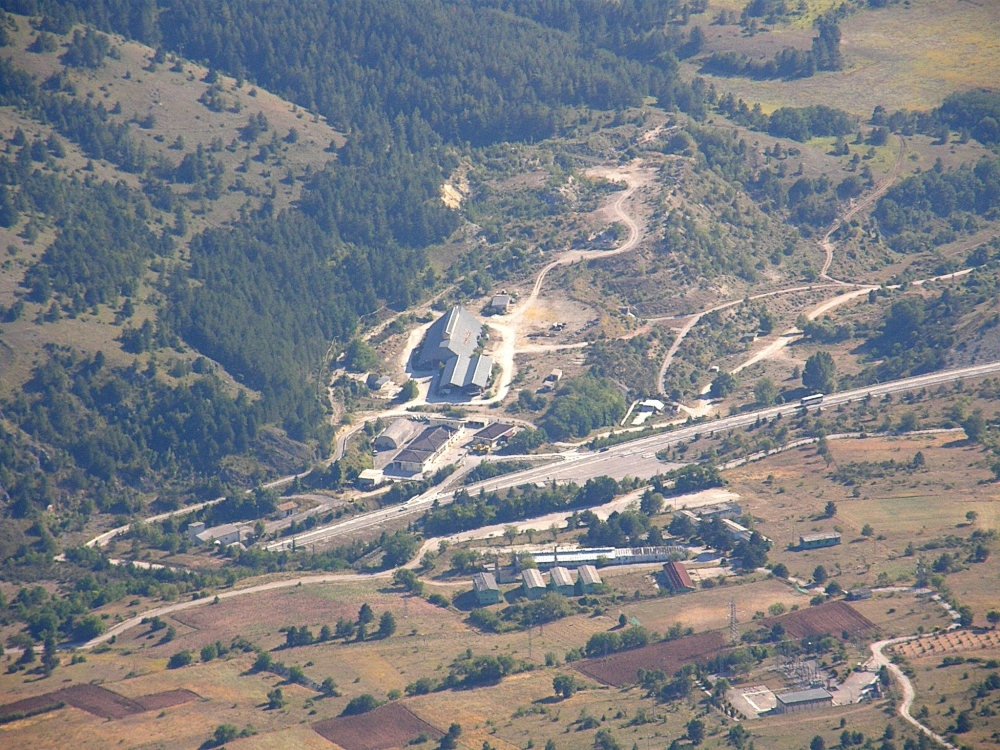
\includegraphics[width=\textwidth]{media/gs.jpg}
	%	\caption*{\href{https://commons.wikimedia.org/w/index.php?curid=4861688}{LNGS -- By Ra Boe (CC BY-SA 3.0)}}
	%\end{figure}
	\begin{figure}
		\centering
		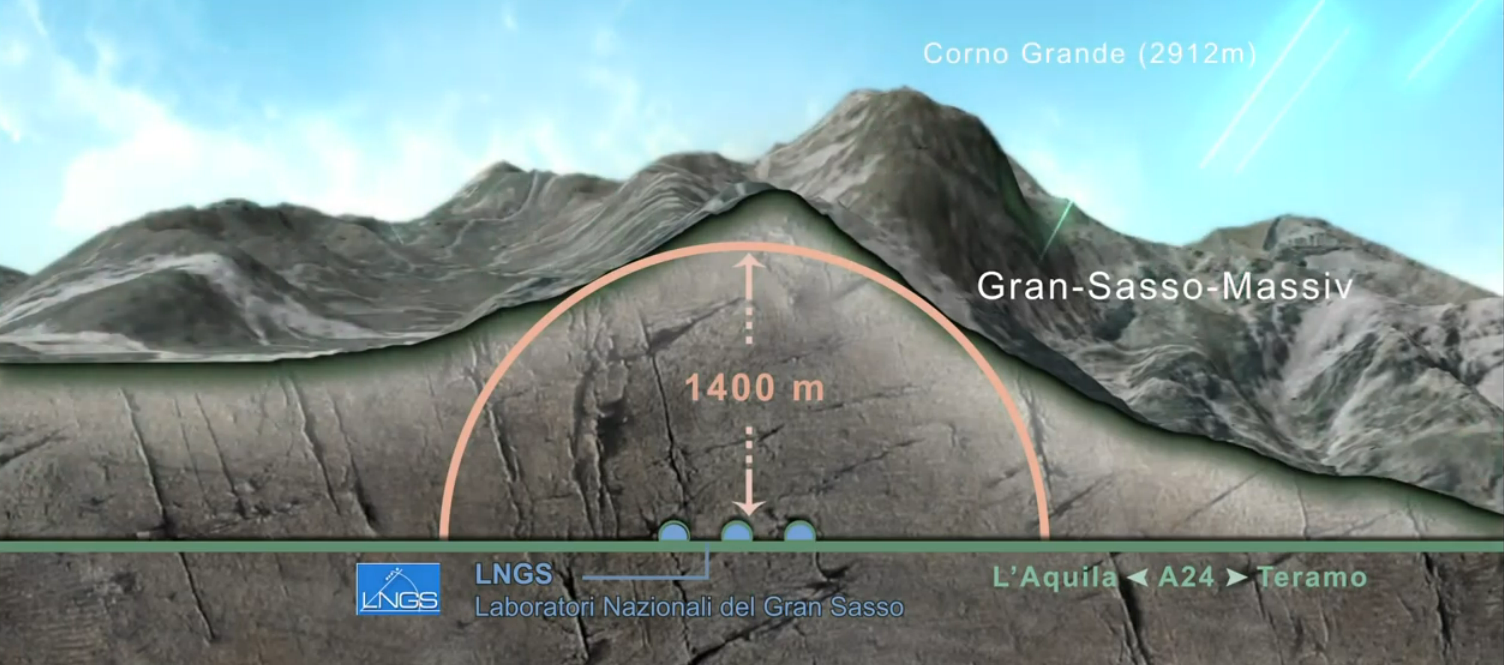
\includegraphics[width=0.5\textwidth]{media/gs_anim.png}
		\caption*{\copyright \href{https://www.cresst.de/video.html}{CRESST collaboration}}
	\end{figure}
\end{frame}
\begin{frame}
	\frametitle{The Heidelberg-Moscow Experiment}
	Back-of-the-envelop calculation of number of $0\nu\beta\beta$ events:
	\begin{align*}
		N_{0\nu}
		= N_{\symup{Ge76}}
		\l(1-
		\exp\l({-\ln{(2)}\frac{t}{T^{0\nu}_{\sfrac{1}{2}}}}\r)
		\r)
		\approx 
		\ln(2)N_{\symup{Ge76}}\frac{t}{T^{0\nu}_{\sfrac{1}{2}}}
	\end{align*}
	\pause
	\centering
	\alert{E.g. $T^{0\nu}_{\sfrac{1}{2}}=\SI{2e25}{\year} \Rightarrow $ \num{5} events per year}
\end{frame}
